\documentclass{amsart}
\usepackage[ruled,vlined]{algorithm2e}
\usepackage{amsmath}
\usepackage[margin=1in]{geometry}
\DeclareMathOperator*{\argmax}{arg\,max}
\DeclareMathOperator*{\argmin}{arg\,min}
\usepackage{ifpdf}
\usepackage{url}
\usepackage{graphicx}
\usepackage{float}
\usepackage{amsfonts}
\title{Project 5 \\ Feedforward Neural Networks}
\author{David Atlas}
\begin{document}
    \begin{abstract}
    This paper will introduce feed-forward neural networks, a
        technique for learning non-linear functions. The backpropogation
        algorithm will be used in conjunction with
        gradient descent. Networks of 0, 1 and 2 hidden layers will be
        applied to several different real-world classification
        problems. The size of the hidden
        layer will be tuned using a validation set.
        A sigmoid activation function will
        be used to introduce non-linearities into the network.
        A softmax classifier will be used to train a multi-net
        classifier. The networks mostly outperform
        a naive baseline, although require
        substantial tuning effort to converge to a good solution.
    \end{abstract}
    \maketitle

    \section{Problem Statement \& Hypothesis}
    Feed-forward neural networks are a popular technique for estimating
    non-linear relationships between a set of inputs, and the densities of a
    corresponding class label or regression target. In a feed-forward
    neural network, an affine transformation is conducted on
    an input, at which point a non-linear function (which will be
    called an activation function) is applied. This is the basic
    unit of a network. Many of these units can be combined, with
    the effect being a flexible model that can learn non-linearities
    and feature interactions.

    Therefore, the hypothesis is that the networks should outperform
    naive baselines across all the real-world experiments run in
    this paper, as it is known from previous experiments that
    a simple linear classifier can outperform baseline on these
    problems. As such, the feed-forward network has \textit{at least}
    as much capacity as those models, and should outperform.

    However, the additional cost of the expanded model
    capacity is that the networks can be difficult to train.
    They are sensitive to the learning rate, number of iterations
    and size of each of the units. Therefore, it would not be
    wholly unexpected if it were to be too difficult to find
    a network that outperforms a simpler linear model
    on problems with classes that are largely linearly seperable.

    In the experiments below, 3 network configurations are used.
    A network with 0, 1 and 2 hidden layers will be applied to
    each problem. It is expected that the network with no hidden
    layers will perform in-line or better that the networks with
    hidden layers on problems with linear seperability. If an
    experiment presents a non-linear boundary between classes,
    it is expected that the hidden layer networks will outperform.

    \section{Description of Algorithms}
    \subsection*{Single Unit}
    The networks discussed in this paper are all composed of
    simple, small units. Each unit takes an input $X$ and
    generates an output $z$ via the following function:
    \begin{align*}
        \sigma(x) = \frac{1}{1 + \exp{-x}}
        z &= \sigma(XW) \\
    \end{align*}
    where $W$ is a matrix with the same number of rows as $X$
    has columns. $sigma(x)$ is the sigmoid activation function, shown
    below in Figure~\ref{sigmoid}.
    \begin{figure}
        \centering
        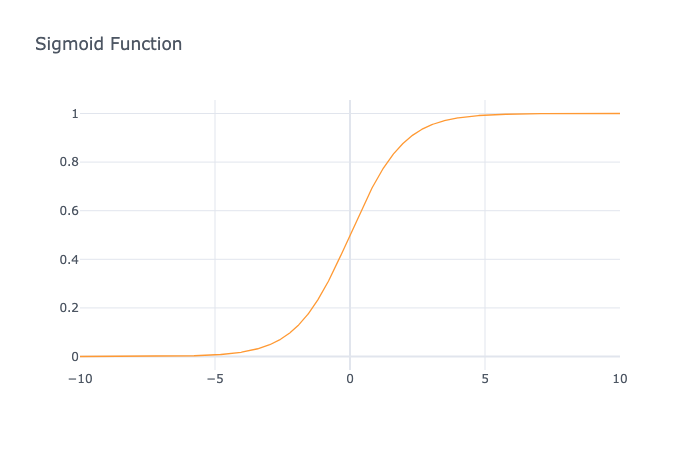
\includegraphics[width=.6\textwidth]{sigmoid.png}
        \label{sigmoid}
    \end{figure}
    The sigmoid function plays two roles in the network. First, it
    introduces non-linearity. This is important, because several
    sequential linear transformations create a linear transformation,
    meaning that the network would only be able to create
    linear functions. Adding in the sigmoidal activation
    changes that. Second, the function maps from an unbounded space to
    the $[0, 1]$ interval. When training a classifier, the output
    must be interpreted as binary. The output of the sigmoid
    function can be interpreted as the probability of a positive
    predictions. This is also advantageos relative to a binary label
    because the interpretation is naturally probablistic.

    \subsection*{Network Topology}
    Now that the basic unit of the network has been established, there
    are two parameters that must be chosen within the network\cite{deeplearning}.

    The number of additional units to include in the network (which will be
    called the hidden layers) is crucial in defining the capacity of the
    network. As the number of units grows, the capacity of the
    network increases, all else equal, which reflects a change in the
    representation bias. However, the search space becomes bigger,
    and the selection bias plays a large role in whether the network
    converges to a performant solution.

    Beyond the number of hidden layers, the size of each
    hidden layer must be chosen.
    Above, $W$ was defined as a $m \times k$ (where $X$ is $n \times m$).
    This leaves $k$ as a parameter. In the experiments conducted here,
    $k$ will be tuned over a validation set.
    Note that the effect of a larger value of $k$ is similar to adding more
    units in the network - larger values will increase the representation
    capacity, but will create more parameters (and thus a larger search space).

    There is also a relationship between the two parameters. A network
    might have fewer large hidden layers, or many small hidden layers.
    Fewer layers may be easier to train, but many layers can give more capacity
    with fewer parameters. Both should be chosen based on the problem.

    \subsection*{Backpropogation}
    Given the network defined above, the challenge is in tuning
    the weight matrices $W_h$ for each of the $h$ units in
    the network. As in past papers, gradient descent will be
    used, but the challenge remains in calculating the gradient\cite{backprop}.
    Given the loss function
    \[
        E(W, X) = (O - Y)^T (O - y)
    \],
    where $o_i \in O$
    is the output of the network given input $X_i$, and $Y$
    is a vector of targets corresponding rowwise to $X$,
    the derivative of the loss relative to the output of the
    network is
    \[
        \frac{dE}{dO} = (O - y).
    \]
    At this point, the chain rule must be
    applied to find the derivative of the loss relative
    to the weights in the final layer.
    The derivative of the sigmoid function is
    \[
        \sigma^\prime (x) = \sigma(x) (1 - \sigma(x)),
    \]
    and so \[
        \frac{dE}{dW_H} =
        \frac{dE}{dO} \frac{\partial O}{\partial W_H} =
        (O - Y) \sigma(X) (1 - \sigma(X)) X.
    \]

    Next, the derivative for each of the preceding units
    must be found. First, $\delta_i$ is defined as
    \[
        \delta_i = -\frac{\partial E}{\partial O_i},
    \]
    where $O_i$ is the output of the $i^{th}$ layer.
    Using the chain rule, this can be written as
    \begin{align*}
        \delta_i &= - \frac{\partial E}{\partial O_{i+1}}
        \frac{\partial O_{i+1}}{\partial O_{i}} \\
        &= \delta_{i+1}  \frac{\partial O_{i+1}}{\partial O_{i}} \\
        &= \delta_{i+1} W_{i+1} \frac{\partial O_i}{\partial X_i} \\
        &= \delta_{i+1} W_{i+1} O_i (1 - O_i).
    \end{align*}

    Practically, the delta rule will be leveraged.
    Rather than recalculating the derivative for each unit,
    the derivative can be expressed as the cumulative effect of
    all the units downstream from a given unit. This cumulative
    effect will be denoted $\delta_j$ for the $j^{th}$ unit in the network:
    \[
        \delta_j = \delta_{j+1} W_{j+1} \circ  O_j (1 - O_j),
    \]
    where $A \circ B$ denotes the Hadamard (element-wise) product of $A$ and $B$,
    and $O_j$ indicates the output of the $j^{th}$ unit. This is where
    the term \textit{backpropogation} comes from - the derivative of the error
    is propogated backwards through each of the preceding units, all without
    having to recalculate the individual quantities, by accumulated
    $\delta_i$ throughout the network.

    \subsection*{Gradient Descent}
    Having presented the delta-rule, calculating the gradient updates is easy.
    \[
        \Delta W_h = \eta \delta_h X_h,
    \]
    where $\eta$ is the learning rate, $\delta_h$ is as defined above (the sum
    over all of the downstream $\delta_i$), and $X_h$ is the input to the $h^{th}$
    unit (the output of the $h-1^{th}$ unit or the original set of features if
    $h=1$).

    This process will repeat iteratively until either some convergence criteria is
    met, or the a specified number of iterations is reached.

    \section{Experimental Approach}
    For each of the 5 real-world experiments conducted, networks with 0, 1 and 2 hidden
    layers were trained. The size of the hidden layers and the
    learning rate were both tuned using a validation set, and chosen based on which
    set minimized the out-of-sample classification error.
    A stratified 5-fold cross-validation scheme was used to estimate
    the out-of-sample error. All problems were trained using a multi-net approach, where each
    class label has a corresponding output, and a softmax function was used to calculate
    the error relative to a one-hot encoding of the class labels.

    \section{Experimental Results}
    \subsection*{Breast Cancer Data}
    The first experiment conducted involved the classification of a breast tumor
    as malignant or benign\cite{cancerdataset}. Rows containing null values were dropped, as they're a small portion of the
    data. The features were also mean-centered at zero and scaled by the standard deviation.
    As mentioned above, a cross-validation approach was used to pick the size of the hidden layers and
    the learning rate. Batches of size 48 were, providing some stability in the learning process.
    The results of the experiments can be found in Table~\ref{breast_results}.
    \begin{table}[H]
    \begin{tabular}{lccc}
    Model & Size of H1 & Size of H2 & Mean Accuracy \\
    \hline
    No Hidden Layer & NA & NA & 97\%\\
    One Hidden Layer & 4 & NA & 97\% \\
    Two Hidden Layers & 4 & 8 & 97\% \\
    Naive Baseline & NA & NA & 65\%
    \end{tabular}
    \label{breast_results}
    \caption{Breast Cancer Classification Results}
    \end{table}


    \subsection*{Soybean Experiment}
    The next experiment run was to classify the type of rot exhibited by a soybean given
    characteristics about the bean\cite{soybeandataset}. As above, cross-validation was used to determine the best
    size of both of the hidden layers and the learning rate. A batch size of 48 was used again.
    The network with no hidden layer performed quite well, while the networks with hidden layers
    perform in line with a naive baseline. The results can be found in Table~\ref{soybean_results}.
    \begin{table}[H]
    \begin{tabular}{lccc}
    Model & Size of H1 & Size of H2 & Mean Accuracy \\
    \hline
    No Hidden Layer & NA & NA & 98\%  \\
    One Hidden Layer & 5 & NA & 36\% \\
    Two Hidden Layers & 7 & 9 & 36\% \\
    Naive Baseline & NA & NA & 36\%
    \end{tabular}
    \label{soybean_results}
    \end{table}

    \subsection*{Iris Experiment}
    The Iris dataset\cite{irisdataset} involves classifying the type of flower based on measurements
    of the flower. As above, cross-validation was used to find the size of the hidden layers and the learning
    rate. A batch size of 48 was used. The networks had some trouble converging to extremely
    performant results, but all were able to outperform the baseline naive model on average.
    The experiment results can be found in Table~\ref{iris_results}.
    \begin{table}[H]
    \begin{tabular}{lccc}
    Model & Size of H1 & Size of H2 & Mean Accuracy \\
    \hline
    No Hidden Layer & NA & NA & 74\% \\
    One Hidden Layer & 4 & NA & 66\% \\
    Two Hidden Layers & 3 & 4 & 66\% \\
    Naive Baseline & NA & NA & 33\%
    \end{tabular}
    \label{iris_results}
    \end{table}

\bibliographystyle{plainurl}
\bibliography{biblio}
\end{document}